\subsection{Electromagnetic Calorimeter} 
\label{sec:ecal}

The Ecal, depicted in Fig. \ref{fig:ecal}, consists of $442$ lead-tungstate PbWO$_4$ crystals with avalanche photodiode (APD) readout and amplifiers. Those have all similarly short pulse widths, so that they can run at very high rates. Indeed, the expected high radiation and high rate environment, together with a high magnetic field in close proximity, essentially imposed lead-tungstate (PbWO$_4$) crystals with APD readout. The lead tungsten (PbWO$_4$) crystals are taken from the Inner Calorimeter (IC) of the JLab CLAS detector, which was originally build in IPN Orsay and run for 10 years with success. Crystals in the ECal are arranged in two modules. There are 5 layers in each module; four layers have $46$ crystals and one has $37$. The ECal is mounted downstream of the analyzing dipole magnet at the distance of about $137$ cm from the upstream edge of the magnet. The two ECal modules are positioned just above and below the ECal vacuum chamber, through which the beam and the wall of flame passes in vacuum. At its closest point, the edge of the crystal is at $3.7$ cm from the beam. In order to maintain stable performance of the PbWO$_4$ calorimeter, the crystals and APDs are enclosed within a temperature stabilized environment, held constant at the level of 1\!\char23F. The expected energy resolution of the system from operational experience with the IC is $\sigma_E/E \sim 4.5\%/\sqrt{E}$ (GeV). As in the IC, PbWO$_4$ modules are connected to a motherboard that provides power and transmits signals from individual APDs and pre-amplifier boards. The ECal data is digitized using the JLAB FADC250, a 250 MHz flash ADC developed for the 12 GeV Upgrade. The full analogue information from the FADCs coupled with the spatial and time information of each module are available to the trigger system, which uses energy deposition, position, timing, and energy-position correlation to reduce the trigger rate to a manageable $\sim 30$ kHz (see section \ref{seq:ECalTrigger} for details).

\begin{figure*}[t]
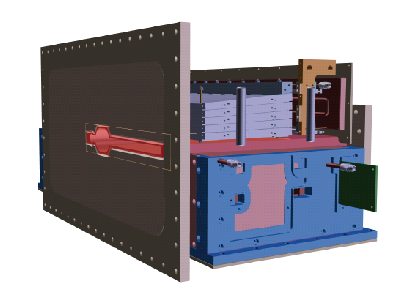
\includegraphics[scale=0.7]{ecal/ECal.png}
\caption{\small{Cut-away view of the Ecal, showing the vacuum flange which mates to the magnet vacuum chamber on the left, holes for the electron beam and the “wall of flame” in the Ecal vacuum chamber (in red), crystal positions in the upper module, and the temperature control box in blue in the lower module.}}\label{fig:ecal}
\end{figure*}

For an experiment like HPS, where backgrounds must be well understood and need to be strongly suppressed, the trigger bias can be an important issue. In particular, having a stable and known thresholds at the trigger readout are necessary in order to avoid the bias in the event selection. The uniformity of trigger response and the stability can be achieved with the installation of an online gain monitoring system. This system will introduce short light pulses in the front of the crystals. Optical fibers will be used to transmit light from the source to the crystals to test the response of APDs. The response of the system will therefore be sensitive to both transparency losses of crystals due to a possible radiation damage and gain variations of APDs. Such a system has been developed for several experiments (CMS at CERN for instance) with various light sources. The system for ECal will be developed in IPN Orsay during 2013 and in the first half of 2014, to be ready for installation at JLAB for the commissioning run at the end of 2014. We choose, for their low cost, to use two different mono-color LEDs as light sources to monitor responses of each module. A blue light, which corresponds to the domain of the crystal emission, and is very sensitive to the presence of color centers, produced by radiation damage. This light source is very useful to test variations of the response in the main domain of the emission. Impurities can anneal at room temperature and such monitoring can be sensitive to increasing of output as well, when the radiation exposure is reduced for a long period of time. A red colored light, less sensitive to the color centers, permits monitoring the APD gains more directly and thereby separates effects of APD and electronics from the crystal transparency, and provide clear information on the state of the electronics. The main challenge for the system is to guarantee stability at a level better than a couple percent to be able to identify and to adapt to the transparency variations. The test of the system will be carried-on at IPN Orsay, in order to guarantee its efficiency and also to test radiation resistance of the various materials.

The second major improvement to be done for the calorimeter consists in the implementation of new APDs, by replacing old $5\times 5$ mm$^2$ APDs with $10\times 10$ mm$^2$, Hamamatsu S8664-1010. The renewal of the APDs will resolve two issues with present modules of HPS calorimeter. First, new APDs from Hamamatsu have much better performance than the ones which are now installed on lead-tungstate crystals. Data from Hamamatsu shows that APDs made from the same wafer have excellent uniformity. With $\pm 10\%$ known uniformity at the gain of $100$, variations in bias voltage are $\sim 4.5$ V. Moreover, data provided for samples of 1300 the bias voltage difference is ~50 V, when for APDs now we have ($442$ pieces) the voltage difference is more than $100$ V. So, it is clear that with new APDs much better uniformity in the response of the calorimeter modules in the trigger can be achieved. Second, $4$ times larger readout area will ensure $4$ times more light collection and therefore $4$ time larger signal from APDs. This will allow the use of different amplifier modules with lower gain that in turn will decrease electronic noise. Tests performed for another calorimeter, now in production at INFN Genova for JLAB Hall-B, showed that the same type of amplifier boards with factor 2 lower gains have noise level on the order of $<5$ MeV. Minimum ionizing energy deposition in PbWO$_4$ crystals of HPS calorimeter from cosmic muons passing through perpendicular to the crystal axis is of $\sim 15$ MeV. If energy thresholds can be moved close to $5$ MeV, then MIP peak will be seen and calorimeter can be calibrated and monitored with cosmic muons. The INFN group made the first tests with HPS crystals using Hamamtsu $10\times 10$ mm$^2$ APDs and the new amplifier boards. In Figure \ref{fig:mip10x10} charge distribution of the single crystal system is shown. The red line histogram is for all events triggered by scintillation telescope located above and below the crystal. The black line histogram corresponds to charge distribution within $100$ ns of coincidence time. The MIP peak is clearly visible and well isolated from the pedestal (noise). The same crystal with old $5\times 5$ mm$^2$ APD also gets the signal from MIP, but the MIP charge distribution is under the noise peak and does not have well defined peak position, see Figure \ref{fig:mip5x5}. Possibility of detecting MIP particles traversing the system in perpendicular direction will allow to calibrate the modules with cosmic muons while they are installed in the detector. This is a great advantage and together with light monitoring system will ensure stable and reliable performance of the ECal and the trigger system. In addition to the possibility of calibrating the modules with cosmic muons (MIP calibration), the lower noise will allow to lower the acquisition thresholds and improve the energy resolution. The new amplifier boards have to be designed to work with new APDs. IPN Orsay will design the new boards in collaboration with JLAB. 

\begin{figure*}[t]
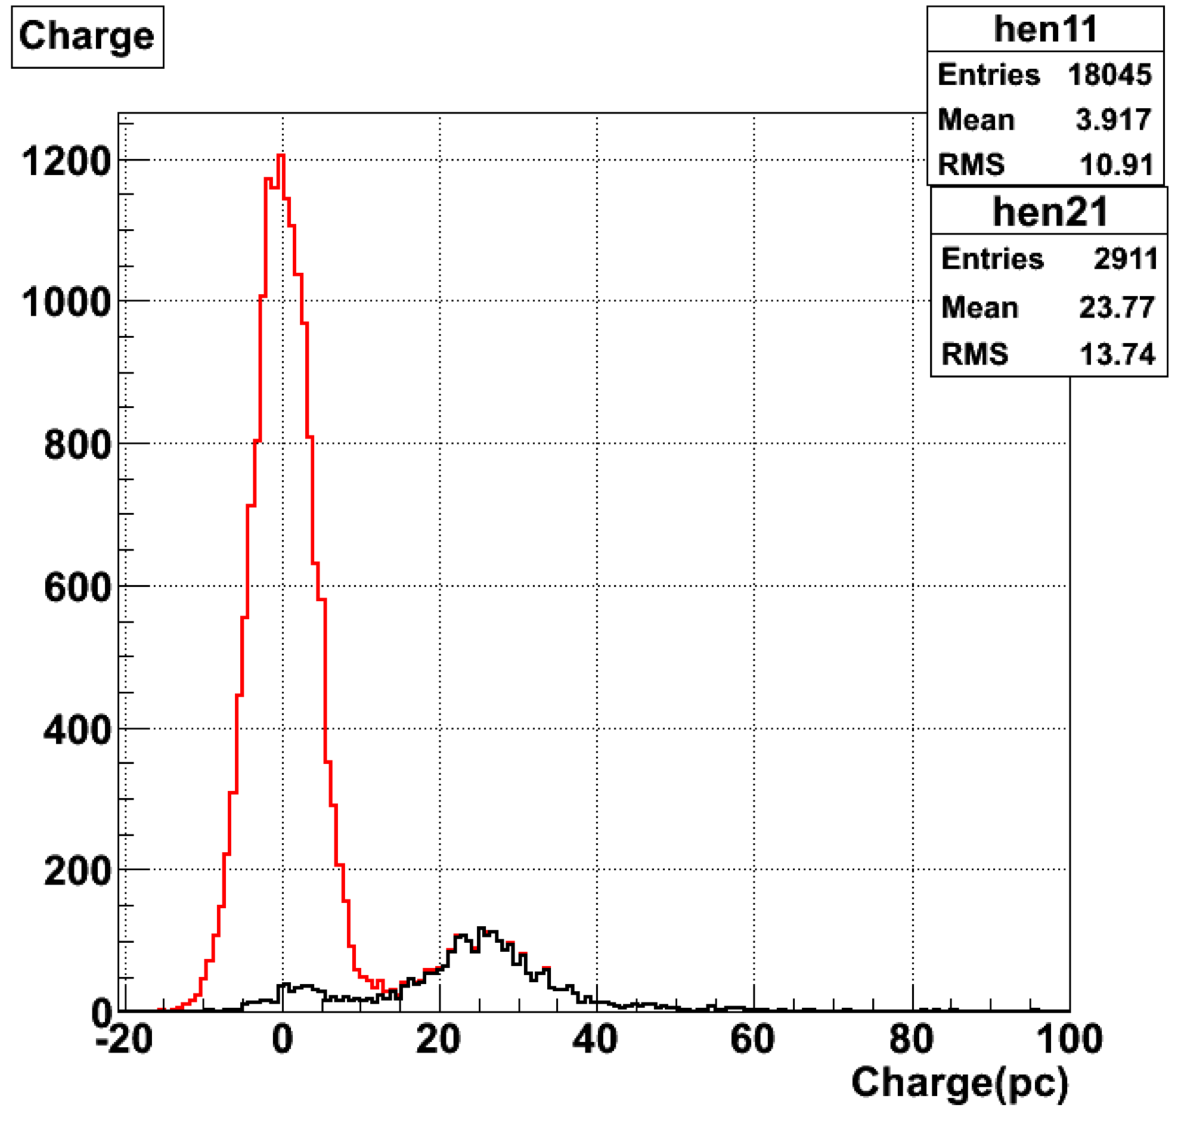
\includegraphics[scale=0.5]{ecal/MIP_10x10_APD.png}
\caption{\small{Charge distribution on QDC from readout of the HPS calorimeter crystal with Hamamatsu S8664-1010 APD and the new low noise amplifier board. The red line histogram corresponds to all events, while the black line distribution is for events within $100$ ns of the trigger signal from the scintillation telescope.}}\label{fig:mip10x10}
\end{figure*}

\begin{figure*}[t]
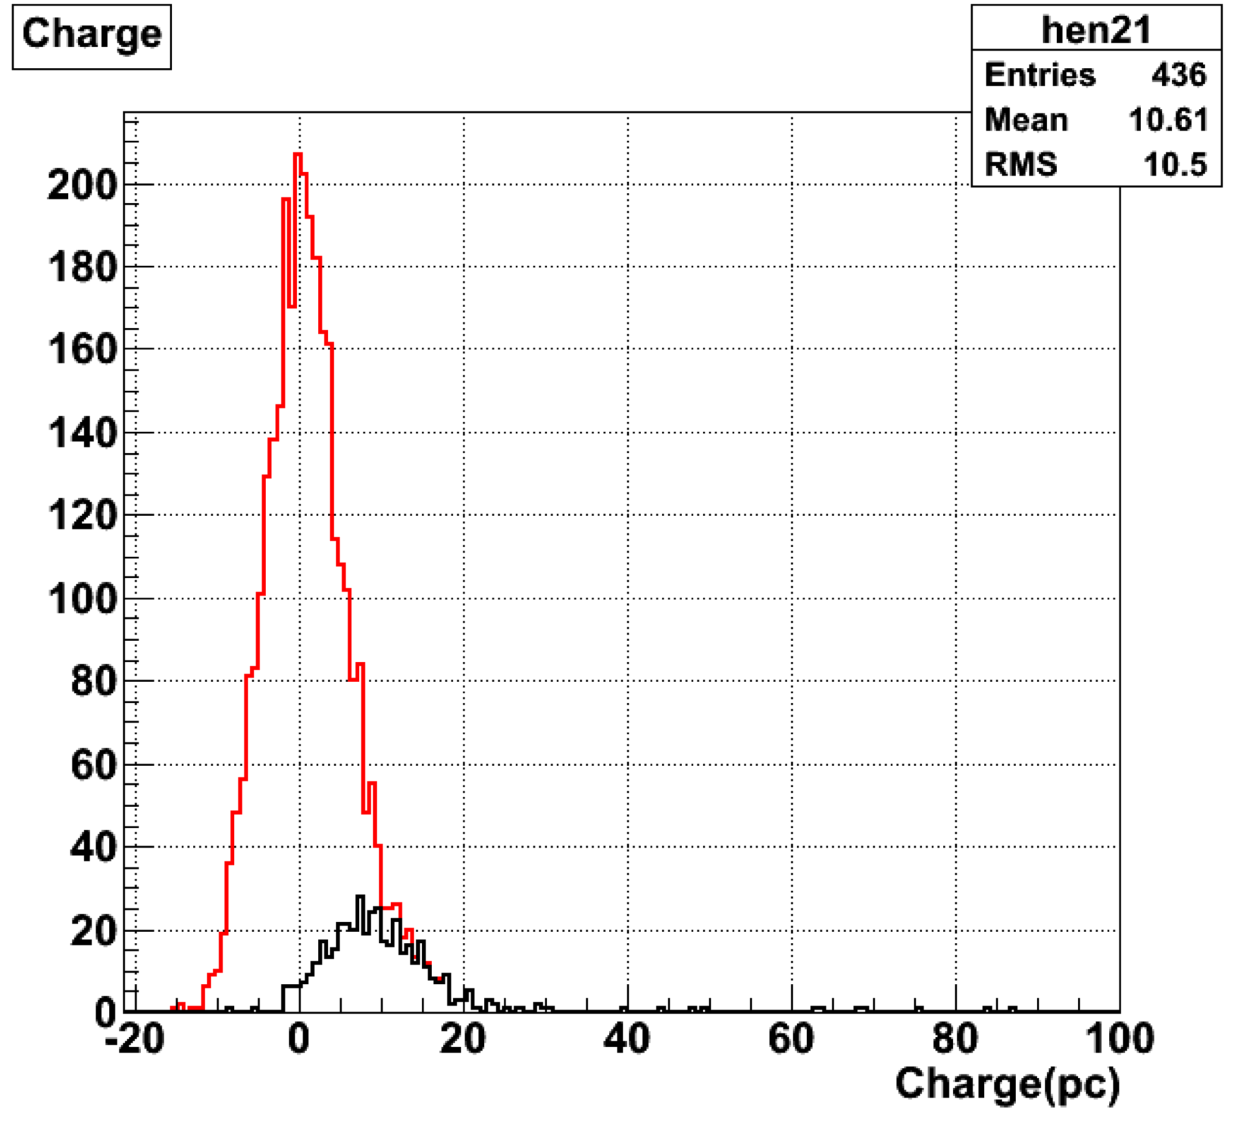
\includegraphics[scale=0.5]{ecal/MIP_5x5_APD.png}
\caption{\small{The same as in Figure \ref{fig:mip10x10} but for readout with currently used $5\times 5$ mm$^2$ APD.}}\label{fig:mip5x5}
\end{figure*}
